% Created by tikzDevice version 0.12.3 on 2020-06-03 12:05:44
% !TEX encoding = UTF-8 Unicode
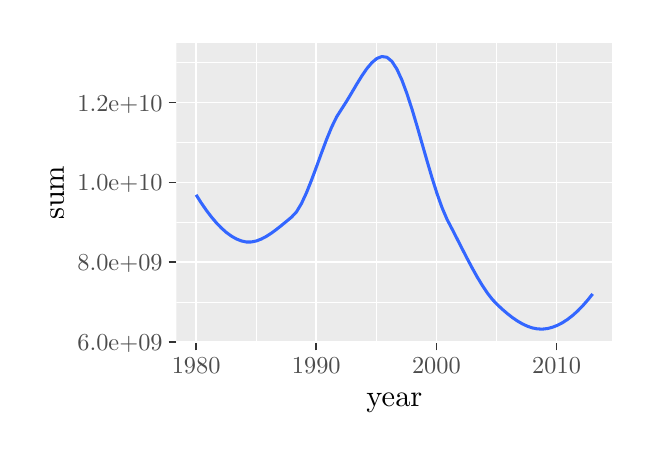
\begin{tikzpicture}[x=1pt,y=1pt]
\definecolor{fillColor}{RGB}{255,255,255}
\path[use as bounding box,fill=fillColor,fill opacity=0.00] (0,0) rectangle (216.81,144.54);
\begin{scope}
\path[clip] (  0.00,  0.00) rectangle (216.81,144.54);
\definecolor{drawColor}{RGB}{255,255,255}
\definecolor{fillColor}{RGB}{255,255,255}

\path[draw=drawColor,line width= 0.6pt,line join=round,line cap=round,fill=fillColor] (  0.00,  0.00) rectangle (216.81,144.54);
\end{scope}
\begin{scope}
\path[clip] ( 53.71, 30.69) rectangle (211.31,139.04);
\definecolor{fillColor}{gray}{0.92}

\path[fill=fillColor] ( 53.71, 30.69) rectangle (211.31,139.04);
\definecolor{drawColor}{RGB}{255,255,255}

\path[draw=drawColor,line width= 0.3pt,line join=round] ( 53.71, 45.37) --
	(211.31, 45.37);

\path[draw=drawColor,line width= 0.3pt,line join=round] ( 53.71, 74.20) --
	(211.31, 74.20);

\path[draw=drawColor,line width= 0.3pt,line join=round] ( 53.71,103.04) --
	(211.31,103.04);

\path[draw=drawColor,line width= 0.3pt,line join=round] ( 53.71,131.88) --
	(211.31,131.88);

\path[draw=drawColor,line width= 0.3pt,line join=round] ( 82.58, 30.69) --
	( 82.58,139.04);

\path[draw=drawColor,line width= 0.3pt,line join=round] (126.00, 30.69) --
	(126.00,139.04);

\path[draw=drawColor,line width= 0.3pt,line join=round] (169.41, 30.69) --
	(169.41,139.04);

\path[draw=drawColor,line width= 0.6pt,line join=round] ( 53.71, 30.95) --
	(211.31, 30.95);

\path[draw=drawColor,line width= 0.6pt,line join=round] ( 53.71, 59.79) --
	(211.31, 59.79);

\path[draw=drawColor,line width= 0.6pt,line join=round] ( 53.71, 88.62) --
	(211.31, 88.62);

\path[draw=drawColor,line width= 0.6pt,line join=round] ( 53.71,117.46) --
	(211.31,117.46);

\path[draw=drawColor,line width= 0.6pt,line join=round] ( 60.87, 30.69) --
	( 60.87,139.04);

\path[draw=drawColor,line width= 0.6pt,line join=round] (104.29, 30.69) --
	(104.29,139.04);

\path[draw=drawColor,line width= 0.6pt,line join=round] (147.70, 30.69) --
	(147.70,139.04);

\path[draw=drawColor,line width= 0.6pt,line join=round] (191.12, 30.69) --
	(191.12,139.04);
\definecolor{drawColor}{RGB}{51,102,255}

\path[draw=drawColor,line width= 1.1pt,line join=round] ( 60.87, 84.14) --
	( 62.68, 81.28) --
	( 64.50, 78.64) --
	( 66.31, 76.24) --
	( 68.13, 74.09) --
	( 69.94, 72.20) --
	( 71.75, 70.58) --
	( 73.57, 69.25) --
	( 75.38, 68.22) --
	( 77.19, 67.49) --
	( 79.01, 67.09) --
	( 80.82, 67.10) --
	( 82.63, 67.47) --
	( 84.45, 68.17) --
	( 86.26, 69.13) --
	( 88.07, 70.30) --
	( 89.89, 71.63) --
	( 91.70, 73.07) --
	( 93.52, 74.56) --
	( 95.33, 76.06) --
	( 97.14, 77.99) --
	( 98.96, 81.04) --
	(100.77, 84.95) --
	(102.58, 89.49) --
	(104.40, 94.38) --
	(106.21, 99.37) --
	(108.02,104.19) --
	(109.84,108.60) --
	(111.65,112.33) --
	(113.47,115.18) --
	(115.28,118.01) --
	(117.09,121.04) --
	(118.91,124.12) --
	(120.72,127.06) --
	(122.53,129.70) --
	(124.35,131.87) --
	(126.16,133.40) --
	(127.97,134.11) --
	(129.79,133.85) --
	(131.60,132.38) --
	(133.42,129.56) --
	(135.23,125.60) --
	(137.04,120.71) --
	(138.86,115.13) --
	(140.67,109.08) --
	(142.48,102.77) --
	(144.30, 96.43) --
	(146.11, 90.29) --
	(147.92, 84.56) --
	(149.74, 79.48) --
	(151.55, 75.25) --
	(153.37, 71.76) --
	(155.18, 68.22) --
	(156.99, 64.66) --
	(158.81, 61.13) --
	(160.62, 57.71) --
	(162.43, 54.46) --
	(164.25, 51.45) --
	(166.06, 48.73) --
	(167.87, 46.39) --
	(169.69, 44.47) --
	(171.50, 42.79) --
	(173.31, 41.23) --
	(175.13, 39.81) --
	(176.94, 38.57) --
	(178.76, 37.51) --
	(180.57, 36.66) --
	(182.38, 36.04) --
	(184.20, 35.69) --
	(186.01, 35.61) --
	(187.82, 35.82) --
	(189.64, 36.29) --
	(191.45, 37.00) --
	(193.26, 37.94) --
	(195.08, 39.12) --
	(196.89, 40.52) --
	(198.71, 42.15) --
	(200.52, 44.00) --
	(202.33, 46.06) --
	(204.15, 48.32);
\end{scope}
\begin{scope}
\path[clip] (  0.00,  0.00) rectangle (216.81,144.54);
\definecolor{drawColor}{gray}{0.30}

\node[text=drawColor,anchor=base east,inner sep=0pt, outer sep=0pt, scale=  0.88] at ( 48.76, 27.92) {6.0e+09};

\node[text=drawColor,anchor=base east,inner sep=0pt, outer sep=0pt, scale=  0.88] at ( 48.76, 56.76) {8.0e+09};

\node[text=drawColor,anchor=base east,inner sep=0pt, outer sep=0pt, scale=  0.88] at ( 48.76, 85.59) {1.0e+10};

\node[text=drawColor,anchor=base east,inner sep=0pt, outer sep=0pt, scale=  0.88] at ( 48.76,114.43) {1.2e+10};
\end{scope}
\begin{scope}
\path[clip] (  0.00,  0.00) rectangle (216.81,144.54);
\definecolor{drawColor}{gray}{0.20}

\path[draw=drawColor,line width= 0.6pt,line join=round] ( 50.96, 30.95) --
	( 53.71, 30.95);

\path[draw=drawColor,line width= 0.6pt,line join=round] ( 50.96, 59.79) --
	( 53.71, 59.79);

\path[draw=drawColor,line width= 0.6pt,line join=round] ( 50.96, 88.62) --
	( 53.71, 88.62);

\path[draw=drawColor,line width= 0.6pt,line join=round] ( 50.96,117.46) --
	( 53.71,117.46);
\end{scope}
\begin{scope}
\path[clip] (  0.00,  0.00) rectangle (216.81,144.54);
\definecolor{drawColor}{gray}{0.20}

\path[draw=drawColor,line width= 0.6pt,line join=round] ( 60.87, 27.94) --
	( 60.87, 30.69);

\path[draw=drawColor,line width= 0.6pt,line join=round] (104.29, 27.94) --
	(104.29, 30.69);

\path[draw=drawColor,line width= 0.6pt,line join=round] (147.70, 27.94) --
	(147.70, 30.69);

\path[draw=drawColor,line width= 0.6pt,line join=round] (191.12, 27.94) --
	(191.12, 30.69);
\end{scope}
\begin{scope}
\path[clip] (  0.00,  0.00) rectangle (216.81,144.54);
\definecolor{drawColor}{gray}{0.30}

\node[text=drawColor,anchor=base,inner sep=0pt, outer sep=0pt, scale=  0.88] at ( 60.87, 19.68) {1980};

\node[text=drawColor,anchor=base,inner sep=0pt, outer sep=0pt, scale=  0.88] at (104.29, 19.68) {1990};

\node[text=drawColor,anchor=base,inner sep=0pt, outer sep=0pt, scale=  0.88] at (147.70, 19.68) {2000};

\node[text=drawColor,anchor=base,inner sep=0pt, outer sep=0pt, scale=  0.88] at (191.12, 19.68) {2010};
\end{scope}
\begin{scope}
\path[clip] (  0.00,  0.00) rectangle (216.81,144.54);
\definecolor{drawColor}{RGB}{0,0,0}

\node[text=drawColor,anchor=base,inner sep=0pt, outer sep=0pt, scale=  1.10] at (132.51,  7.64) {year};
\end{scope}
\begin{scope}
\path[clip] (  0.00,  0.00) rectangle (216.81,144.54);
\definecolor{drawColor}{RGB}{0,0,0}

\node[text=drawColor,rotate= 90.00,anchor=base,inner sep=0pt, outer sep=0pt, scale=  1.10] at ( 13.08, 84.86) {sum};
\end{scope}
\end{tikzpicture}
